\documentclass[12pt,a4paper]{article}
\usepackage[utf8]{inputenc}
\usepackage[vietnamese]{babel}
\usepackage{geometry}
\geometry{top=2cm, bottom=2cm, left=2.5cm, right=2cm}

\usepackage{booktabs}
\usepackage{xltabular}
\usepackage{xcolor}
\usepackage{colortbl}
\usepackage{hyperref}
\usepackage{graphicx}
\usepackage{enumitem}
\usepackage{tcolorbox}
\usepackage{amsmath,amssymb}
\usepackage{fancyhdr}
\usepackage{float}
\usepackage{caption}
\captionsetup[table]{position=top,skip=6pt}
\captionsetup[figure]{position=bottom,skip=6pt}

% Thiết lập màu sắc chuyên nghiệp
\definecolor{brandblue}{RGB}{37, 99, 235}
\definecolor{darkslate}{RGB}{30, 41, 59}
\definecolor{tableheader}{RGB}{239, 246, 255}
\definecolor{lightgray}{RGB}{248, 250, 252}

% Cấu hình Header & Footer
\pagestyle{fancy}
\fancyhf{}
\fancyhead[L]{\small \textcolor{darkslate}{\textbf{BrewLite} -- Sơ Đồ Lớp Miền Nghiệp Vụ (Class Diagram)}}
\fancyhead[R]{\small \textcolor{darkslate}{Task 2.3}}
\fancyfoot[C]{\thepage}
\renewcommand{\headrulewidth}{0.4pt}
\setlength{\headheight}{14pt}

% Cấu hình liên kết
\hypersetup{
    colorlinks=true,
    linkcolor=brandblue,
    urlcolor=brandblue,
    citecolor=brandblue
}

\begin{document}

% Tiêu đề tài liệu
\begin{center}
    {\LARGE \textbf{\textcolor{brandblue}{THIẾT KẾ SƠ ĐỒ LỚP MIỀN NGHIỆP VỤ}}}\\[0.3cm]
    {\large \textbf{(Domain Class Diagram -- UML 2.5 Specification)}}\\[0.4cm]
    \begin{tcolorbox}[colback=lightgray,colframe=brandblue,arc=3mm,width=0.95\textwidth]
        \small
        \textbf{Dự án:} Hệ thống Đặt đồ uống trực tuyến BrewLite\\
        \textbf{Học phần:} Công nghệ Phần mềm (Software Engineering) -- Assignment 2\\
        \textbf{Mã nhiệm vụ:} Task 2.3 \hfill \textbf{Mã truy vết:} Class-01\\
        \textbf{Tệp nguồn PlantUML:} \href{run:class-diagram.puml}{\texttt{docs/diagrams/class-diagram.puml}}\\
        \textbf{Tệp ảnh vector SVG:} \href{run:class-diagram.svg}{\texttt{docs/diagrams/class-diagram.svg}}
    \end{tcolorbox}
\end{center}

\vspace{0.2cm}

\section{Tổng quan mục tiêu \& Tiêu chí nghiệm thu}

Tài liệu này hiện thực hóa Task 2.3 của đồ án BrewLite, xây dựng sơ đồ lớp ở mức Domain Model (mô hình miền nghiệp vụ). Sơ đồ mô tả cấu trúc dữ liệu tĩnh, các thực thể kinh doanh, mối quan hệ cấu trúc, ràng buộc đa số (multiplicity), và các kiểu liệt kê trạng thái (enumerations).

\section{Sơ đồ Lớp miền nghiệp vụ (Domain Class Diagram)}

Sơ đồ được thiết kế bằng ngôn ngữ mô hình hóa PlantUML chuẩn UML 2.5:

\begin{figure}[H]
    \centering
    \IfFileExists{class-diagram.png}{%
        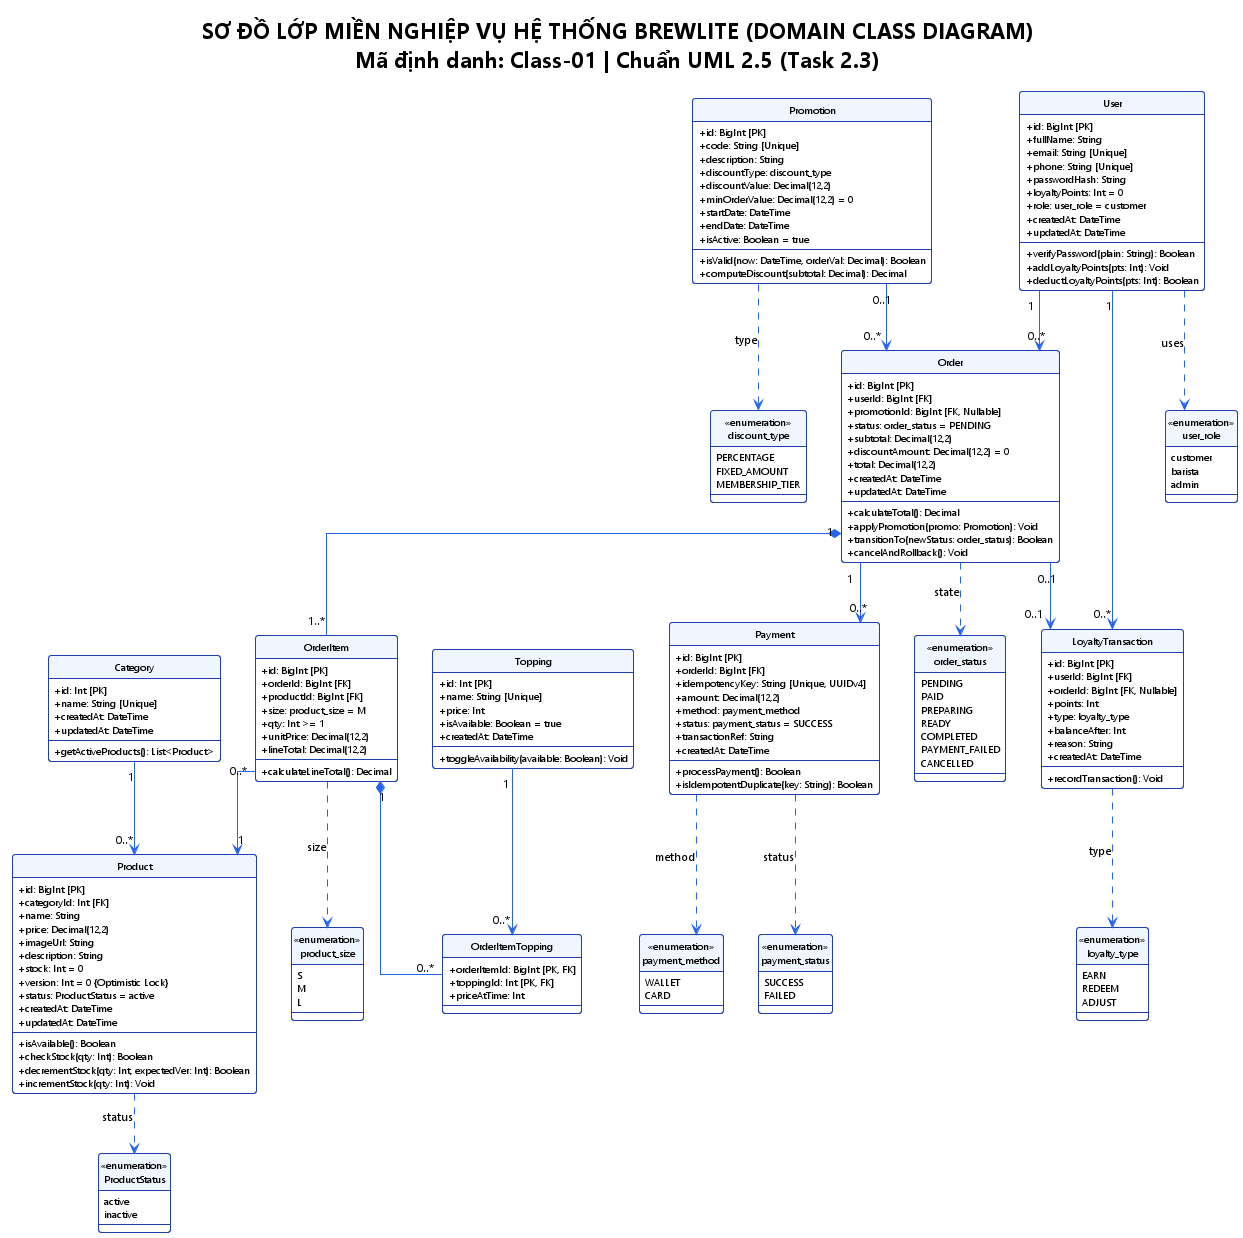
\includegraphics[width=\textwidth]{class-diagram.png}
    }{%
        \fbox{\begin{minipage}{0.95\textwidth}
            \centering
            \vspace{0.5cm}
            \textbf{Sơ đồ Lớp Miền Nghiệp Vụ BrewLite (Class-01)}\\[0.2cm]
            \textit{(Tệp đồ họa vector sắc nét lưu tại: \texttt{docs/diagrams/class-diagram.svg})}\\[0.2cm]
            Mô hình hóa 10 thực thể miền, 8 Enumerations trạng thái, cùng các quan hệ Composition và Association hoàn chỉnh.
            \vspace{0.5cm}
        \end{minipage}}
    }
    \caption{Sơ đồ Lớp Miền Nghiệp Vụ Hệ Thống BrewLite (UML 2.5)}
    \label{fig:class-diagram}
\end{figure}

\section{Đặc tả chi tiết các Lớp Miền Nghiệp Vụ (Domain Entities)}

Hệ thống bao gồm **10 thực thể** (đáp ứng trọn vẹn 7 thực thể bắt buộc của đề bài cùng 3 thực thể hỗ trợ danh mục và topping theo mã nguồn thực tế):

\vspace{0.2cm}
\noindent
\footnotesize
\renewcommand{\arraystretch}{1.25}
\begin{xltabular}{\textwidth}{|c|>{\raggedright\arraybackslash}p{3.4cm}|>{\raggedright\arraybackslash}p{4.2cm}|>{\raggedright\arraybackslash}X|}
\caption{Danh mục 10 Lớp Miền Nghiệp Vụ trong Hệ Thống} \label{tab:classes} \\
\hline
\rowcolor{tableheader}
\textbf{STT} & \textbf{Tên Lớp} & \textbf{Thuộc tính chính \& Kiểu dữ liệu} & \textbf{Phương thức nghiệp vụ chính} \\
\hline
\endfirsthead

\hline
\rowcolor{tableheader}
\textbf{STT} & \textbf{Tên Lớp} & \textbf{Thuộc tính chính \& Kiểu dữ liệu} & \textbf{Phương thức nghiệp vụ (tiếp theo)} \\
\hline
\endhead

\hline
\endfoot

\hline
\endlastfoot

\textbf{1} & \textbf{User}\newline\textit{(Bắt buộc)} & 
\texttt{id: BigInt [PK]}\newline
\texttt{fullName: String}\newline
\texttt{email: String [Unique]}\newline
\texttt{phone: String [Unique]}\newline
\texttt{passwordHash: String}\newline
\texttt{loyaltyPoints: Int = 0}\newline
\texttt{role: user\_role = customer}\newline
\texttt{createdAt, updatedAt: DateTime} & 
\texttt{verifyPassword(plain): Boolean}\newline
\texttt{addLoyaltyPoints(pts): Void}\newline
\texttt{deductLoyaltyPoints(pts): Boolean}\newline
Quản lý tài khoản, mã hóa mật khẩu \texttt{bcrypt} và tích điểm thành viên. \\
\hline

\textbf{2} & \textbf{Product}\newline\textit{(Bắt buộc)} & 
\texttt{id: BigInt [PK]}\newline
\texttt{categoryId: Int [FK]}\newline
\texttt{name: String}\newline
\texttt{price: Decimal(12,2)}\newline
\texttt{imageUrl, description: String}\newline
\texttt{stock: Int = 0}\newline
\texttt{version: Int = 0 \{Lock\}}\newline
\texttt{status: ProductStatus = active}\newline
\texttt{createdAt, updatedAt: DateTime} & 
\texttt{isAvailable(): Boolean}\newline
\texttt{checkStock(qty): Boolean}\newline
\texttt{decrementStock(qty, ver): Boolean}\newline
\texttt{incrementStock(qty): Void}\newline
Quản lý tồn kho đồ uống; kiểm soát tranh chấp bằng khóa lạc quan qua trường \texttt{version}. \\
\hline

\textbf{3} & \textbf{Order}\newline\textit{(Bắt buộc)} & 
\texttt{id: BigInt [PK]}\newline
\texttt{userId: BigInt [FK]}\newline
\texttt{promotionId: BigInt [FK, Null]}\newline
\texttt{status: order\_status = PENDING}\newline
\texttt{subtotal, total: Decimal(12,2)}\newline
\texttt{discountAmount: Decimal(12,2)}\newline
\texttt{createdAt, updatedAt: DateTime} & 
\texttt{calculateTotal(): Decimal}\newline
\texttt{applyPromotion(promo): Void}\newline
\texttt{transitionTo(newStatus): Boolean}\newline
\texttt{cancelAndRollback(): Void}\newline
Thực thi máy trạng thái 7 bước, tính tổng tiền và hoàn trả kho nếu hủy. \\
\hline

\textbf{4} & \textbf{OrderItem}\newline\textit{(Bắt buộc)} & 
\texttt{id: BigInt [PK]}\newline
\texttt{orderId: BigInt [FK]}\newline
\texttt{productId: BigInt [FK]}\newline
\texttt{size: product\_size = M}\newline
\texttt{qty: Int >= 1}\newline
\texttt{unitPrice, lineTotal: Decimal(12,2)} & 
\texttt{calculateLineTotal(): Decimal}\newline
Từng dòng món đặt trong đơn hàng kèm cấu hình dung tích kích cỡ. \\
\hline

\textbf{5} & \textbf{Payment}\newline\textit{(Bắt buộc)} & 
\texttt{id: BigInt [PK]}\newline
\texttt{orderId: BigInt [FK]}\newline
\texttt{idempotencyKey: String [Unique]}\newline
\texttt{amount: Decimal(12,2)}\newline
\texttt{method: payment\_method}\newline
\texttt{status: payment\_status}\newline
\texttt{transactionRef: String}\newline
\texttt{createdAt: DateTime} & 
\texttt{processPayment(): Boolean}\newline
\texttt{isIdempotentDuplicate(key): Boolean}\newline
Xử lý trừ tiền trực tuyến mô phỏng, bảo đảm chống trừ tiền trùng bằng khóa Idempotency duy nhất. \\
\hline

\textbf{6} & \textbf{Promotion}\newline\textit{(Bắt buộc)} & 
\texttt{id: BigInt [PK]}\newline
\texttt{code: String [Unique]}\newline
\texttt{description: String}\newline
\texttt{discountType: discount\_type}\newline
\texttt{discountValue, minOrderValue}\newline
\texttt{startDate, endDate: DateTime}\newline
\texttt{isActive: Boolean = true} & 
\texttt{isValid(now, orderVal): Boolean}\newline
\texttt{computeDiscount(subtotal): Decimal}\newline
Quản lý mã giảm giá và chiết khấu ưu đãi theo hạng thành viên (Bạc, Vàng, Kim Cương). \\
\hline

\textbf{7} & \textbf{LoyaltyTransaction}\newline\textit{(Bắt buộc)} & 
\texttt{id: BigInt [PK]}\newline
\texttt{userId: BigInt [FK]}\newline
\texttt{orderId: BigInt [FK, Nullable]}\newline
\texttt{points: Int}\newline
\texttt{type: loyalty\_type}\newline
\texttt{balanceAfter: Int}\newline
\texttt{reason: String}\newline
\texttt{createdAt: DateTime} & 
\texttt{recordTransaction(): Void}\newline
Lưu vết chi tiết lịch sử cộng/trừ điểm thưởng thành viên (tỷ lệ $10.000$đ = 1 điểm). \\
\hline

\textbf{8} & \textbf{Category} & 
\texttt{id: Int [PK]}\newline
\texttt{name: String [Unique]}\newline
\texttt{createdAt, updatedAt: DateTime} & 
\texttt{getActiveProducts(): List<Product>}\newline
Phân nhóm thực đơn (Cà phê, Trà sữa, Freeze). \\
\hline

\textbf{9} & \textbf{Topping} & 
\texttt{id: Int [PK]}\newline
\texttt{name: String [Unique]}\newline
\texttt{price: Int}\newline
\texttt{isAvailable: Boolean = true}\newline
\texttt{createdAt: DateTime} & 
\texttt{toggleAvailability(status): Void}\newline
Nguyên liệu thêm kèm (trân châu, thạch, kem cheese). \\
\hline

\textbf{10} & \textbf{OrderItemTopping} & 
\texttt{orderItemId: BigInt [PK, FK]}\newline
\texttt{toppingId: Int [PK, FK]}\newline
\texttt{priceAtTime: Int} & 
Liên kết trung gian lưu vết giá topping tại thời điểm khách đặt hàng. \\
\hline
\end{xltabular}

\section{Các kiểu Liệt kê Trạng thái \& Nghiệp vụ (Enumerations)}

\vspace{0.2cm}
\noindent
\small
\renewcommand{\arraystretch}{1.3}
\begin{xltabular}{\textwidth}{|c|>{\raggedright\arraybackslash}p{3cm}|>{\raggedright\arraybackslash}p{4cm}|>{\raggedright\arraybackslash}X|}
\caption{Danh mục 8 Kiểu Liệt Kê (Domain Enumerations)} \label{tab:enums} \\
\hline
\rowcolor{tableheader}
\textbf{STT} & \textbf{Tên Enum} & \textbf{Các giá trị hợp lệ} & \textbf{Ý nghĩa \& Phạm vi áp dụng} \\
\hline
\endfirsthead

\hline
\rowcolor{tableheader}
\textbf{STT} & \textbf{Tên Enum} & \textbf{Các giá trị hợp lệ} & \textbf{Ý nghĩa (tiếp theo)} \\
\hline
\endhead

\hline
\endfoot

\hline
\endlastfoot

\textbf{1} & \texttt{order\_status} & \texttt{PENDING}, \texttt{PAID}, \texttt{PREPARING}, \texttt{READY}, \texttt{COMPLETED}, \texttt{PAYMENT\_FAILED}, \texttt{CANCELLED} & Vòng đời 7 trạng thái của đơn hàng theo máy trạng thái FSM. \\
\hline
\textbf{2} & \texttt{payment\_method} & \texttt{WALLET}, \texttt{CARD} & Phương thức thanh toán mô phỏng (Ví điện tử hoặc Thẻ). \\
\hline
\textbf{3} & \texttt{payment\_status} & \texttt{SUCCESS}, \texttt{FAILED} & Kết quả xử lý trừ tiền từ cổng thanh toán mô phỏng. \\
\hline
\textbf{4} & \texttt{product\_size} & \texttt{S}, \texttt{M}, \texttt{L} & Kích cỡ đồ uống (Size S cơ sở, M $+5.000$đ, L $+10.000$đ). \\
\hline
\textbf{5} & \texttt{ProductStatus} & \texttt{active}, \texttt{inactive} & Trạng thái kinh doanh bật/tắt của món đồ uống. \\
\hline
\textbf{6} & \texttt{user\_role} & \texttt{customer}, \texttt{barista}, \texttt{admin} & Phân quyền truy cập người dùng trong hệ thống (RBAC). \\
\hline
\textbf{7} & \texttt{discount\_type} & \texttt{PERCENTAGE}, \texttt{FIXED\_AMOUNT}, \texttt{MEMBERSHIP\_TIER} & Phân loại hình thức chiết khấu khuyến mãi. \\
\hline
\textbf{8} & \texttt{loyalty\_type} & \texttt{EARN}, \texttt{REDEEM}, \texttt{ADJUST} & Bản chất giao dịch điểm thưởng (Tích điểm khi đơn PAID, Đổi điểm thưởng). \\
\hline
\end{xltabular}

\section{Quan hệ \& Ràng buộc Đa số (Multiplicity)}

Các mối quan hệ cấu trúc tuân thủ nghiêm ngặt ngữ nghĩa UML 2.5:

\begin{itemize}[leftmargin=*,itemsep=3pt]
    \item \textbf{\texttt{Category} $1$ -- $0..*$ \texttt{Product} (Association):} Một danh mục chứa từ 0 đến nhiều sản phẩm. Một sản phẩm thuộc về một danh mục duy nhất.
    \item \textbf{\texttt{User} $1$ -- $0..*$ \texttt{Order} (Association):} Một khách hàng có thể khởi tạo 0 hoặc nhiều đơn hàng.
    \item \textbf{\texttt{Order} $1$ *-- $1..*$ \texttt{OrderItem} (Composition -- Hợp thành sống còn):} Mỗi đơn hàng bắt buộc phải có từ 1 đến nhiều món. Khi đơn hàng bị hủy bỏ triệt để khỏi hệ thống, các \texttt{OrderItem} con tự động bị xóa theo (\texttt{onDelete: Cascade}).
    \item \textbf{\texttt{OrderItem} $1$ *-- $0..*$ \texttt{OrderItemTopping} (Composition):} Mỗi món đồ uống có thể chọn từ 0 đến nhiều loại topping đi kèm.
    \item \textbf{\texttt{Order} $1$ -- $0..*$ \texttt{Payment} (Association):} Một đơn hàng liên kết với các lượt thanh toán. Cho phép lưu vết các lượt thanh toán thất bại (\texttt{PAYMENT\_FAILED}) trước khi có 1 lần thanh toán thành công (\texttt{PAID}).
    \item \textbf{\texttt{Promotion} $0..1$ -- $0..*$ \texttt{Order} (Association):} Một đơn hàng có thể không áp dụng hoặc áp dụng tối đa một mã ưu đãi/chiết khấu thành viên.
    \item \textbf{\texttt{User} $1$ -- $0..*$ \texttt{LoyaltyTransaction} (Association):} Một tài khoản khách hàng sở hữu toàn bộ lịch sử các giao dịch điểm tích lũy.
    \item \textbf{\texttt{Order} $0..1$ -- $0..1$ \texttt{LoyaltyTransaction} (Association):} Mỗi đơn hàng thanh toán thành công (\texttt{PAID}) phát sinh duy nhất một giao dịch cộng điểm thưởng ($10.000\text{đ} = 1\text{ điểm}$).
\end{itemize}

\section{Chứng minh Tiêu chí Nghiệm thu Khắt khe (Zero Contradiction)}

\vspace{0.2cm}
\noindent
\footnotesize
\renewcommand{\arraystretch}{1.25}
\begin{xltabular}{\textwidth}{|c|>{\raggedright\arraybackslash}p{3.8cm}|>{\raggedright\arraybackslash}p{3.8cm}|>{\raggedright\arraybackslash}X|}
\caption{Bảng Đối Chiếu Tính Nhất Quán Tuyệt Đối Của Sơ Đồ Lớp} \label{tab:consistency} \\
\hline
\rowcolor{tableheader}
\textbf{STT} & \textbf{Tài liệu đối chiếu} & \textbf{Điểm ràng buộc kỹ thuật} & \textbf{Minh chứng tính nhất quán trong Class Diagram} \\
\hline
\endfirsthead

\hline
\rowcolor{tableheader}
\textbf{STT} & \textbf{Tài liệu đối chiếu} & \textbf{Điểm ràng buộc kỹ thuật} & \textbf{Minh chứng (tiếp theo)} \\
\hline
\endhead

\hline
\endfoot

\hline
\endlastfoot

\textbf{1} & \textbf{Cơ sở dữ liệu}\newline\path{schema.prisma} & Khóa chính, khóa ngoại, kiểu dữ liệu, trường khóa lạc quan, trường chống trùng thanh toán. & 
Trùng khớp 100\% các kiểu: \texttt{BigInt}, \texttt{Decimal(12,2)}, \texttt{DateTime}.\newline
Trường \texttt{Product.version} thực thi Optimistic Concurrency Control.\newline
Trường \texttt{Payment.idempotencyKey} gán thuộc tính \texttt{[Unique]}. \\
\hline

\textbf{2} & \textbf{Đặc tả yêu cầu (SRS)}\newline\path{srs.md} & Các mã chức năng: FR-01, FR-02, FR-03, FR-05, FR-06, FR-07, FR-08, FR-10, FR-11. & 
FR-01/02 qua \texttt{Product}, \texttt{Category}, \texttt{Topping}.\newline
FR-03 qua \texttt{OrderItem}.\newline
FR-05 qua \texttt{Order.status = PENDING}.\newline
FR-06 qua \texttt{Payment.idempotencyKey}.\newline
FR-07/11 qua \texttt{LoyaltyTransaction} và \texttt{Promotion}.\newline
FR-08 qua \texttt{order\_status} FSM. \\
\hline

\textbf{3} & \textbf{Sơ đồ tuần tự}\newline\path{sequence-checkout.puml} & Thứ tự gọi hàm, transaction tạo đơn và xác thực thanh toán qua cổng mô phỏng. & 
Khớp chính xác các tham số gọi trong Sequence: hàm tạo đơn \texttt{POST /orders} tạo đối tượng \texttt{Order} \& \texttt{OrderItem}; hàm \texttt{POST /payments} kiểm tra trùng \texttt{idempotencyKey} và nạp giao dịch \texttt{LoyaltyTransaction}. \\
\hline

\textbf{4} & \textbf{Sơ đồ hoạt động}\newline\path{activity-order-flow.puml} & Nhánh kiểm tra tồn kho, nhánh hủy đơn và rollback số lượng tồn kho khi thanh toán lỗi. & 
Nhánh kiểm tra tồn kho khớp với \texttt{Product.checkStock()}.\newline
Nhánh hủy đơn quá hạn/thanh toán thất bại khớp với phương thức \texttt{Order.cancelAndRollback()} kích hoạt \texttt{Product.incrementStock()}. \\
\hline
\end{xltabular}

\end{document}
